\chapter{Data, Trigger and Event Selection}

\section{Data}

The search for GMSB described in this thesis uses $1.1 \unit{fb^{-1}}$ of data 
taken from March to June 2011. This corresponds to the data set used for the 
results presented at the International Europhysics Conference in High Energy 
Physics in July 2011. \\

The centre of mass energy of the proton-proton collisions is $7\unit{TeV}$ which
makes the LHC the highest energy particle collider to date. A higher centre of 
mass energy increases the production cross-section of certain processes, for 
example stong production SUSY, and also enables the production of more massive 
particles. It should be noted that the important energy is not the centre of 
mass energy of the proton collision, but that of the parton collision which is 
$\sim 1 \unit{TeV}$ on average. \\

The instantaneous luminosity has increased over the data taking period by 
increasing the intensity of the beams and the number of bunches. Increasing the 
intensity of the beams leads to more interactions per bunch crossing -- an 
effect called pile-up. During the period when this data was taken the luminosity 
was $\sim 10^{33} \unit{cm^{-2}s^{-1}}$. \\

Figure \ref{fig:intlumi} shows the integrated luminosity recorded by CMS over 
time until September 2011. \\

\begin{figure}
\begin{center}
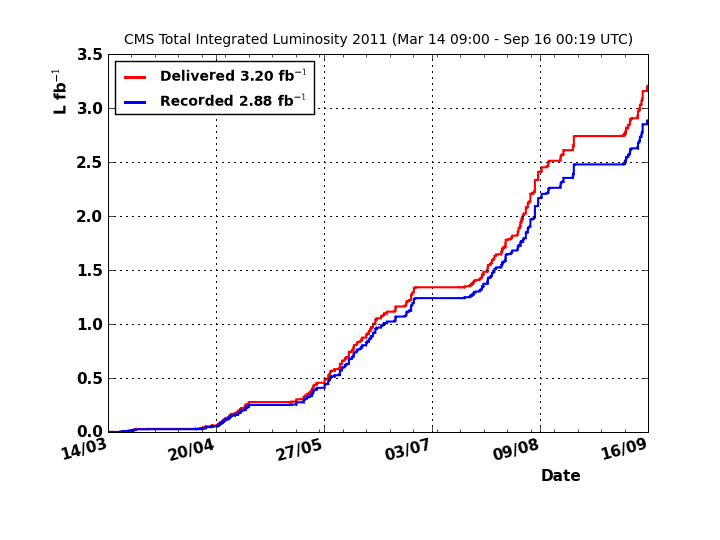
\includegraphics[width=\textwidth]{Integrated_Luminosity.png}
\caption{The integrated luminosity vs time delivered to (red) and recorded by
(blue) CMS during stable beams at $\sqrt{s} = 7 \unit{TeV}$.}
\end{center}
\label{fig:intlumi}
\end{figure}

\section{$\HT$ and Missing Transverse Energy ($\MET$)}

$\HT$ and $\MET$ are two event variables used to search for GMSB in the data. \\ 

$\HT$ is the scalar sum of the $\pT$ of all jets with $\pT > 40\unit{GeV}$.

\begin{equation}
\HT = \sum \pT^{jet}
\end{equation}

$\MET$ is 

\section{Monte Carlo Samples}
\label{sec:Monte_Carlo_Samples}

Event generation using Monte Carlo techniques overlayed with detector simulation
are used to obtain simulated data with which to compare to observations and
validate analysis methods. Monte Carlo samples are generated using Pythia 6 
\cite{pythia6} with Tune Z2 (based on CTECQ6 parton distribution functions 
\cite{tuneZ2}). GEANT \cite{geant} is used for the detector simulation. \\

Pile-up is simulated in the Monte Carlo samples however the MC does not
reproduce the vertex mutiplicity distribution seen in the data. To correctly
simulate pile-up the MC is re-weighted to reproduce the number of vertices
distribution seen in the data. Figure \ref{fig:nVertices} shows the distribution
of number of vertices in the data and MC. Table \ref{tab:factors} gives the 
re-weighting factors for each number of vertices. \\

\begin{figure}
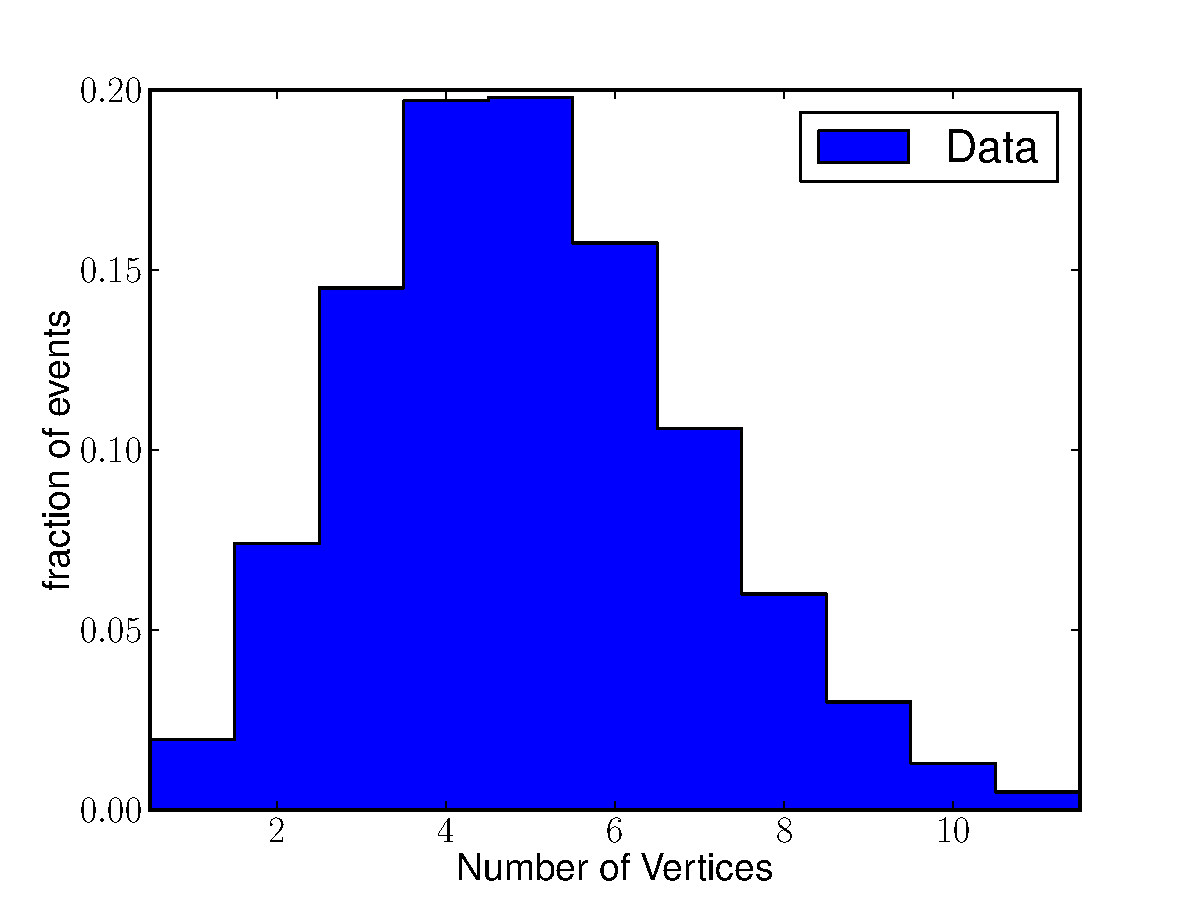
\includegraphics[width=0.5\textwidth]{nVertices_Data.pdf}
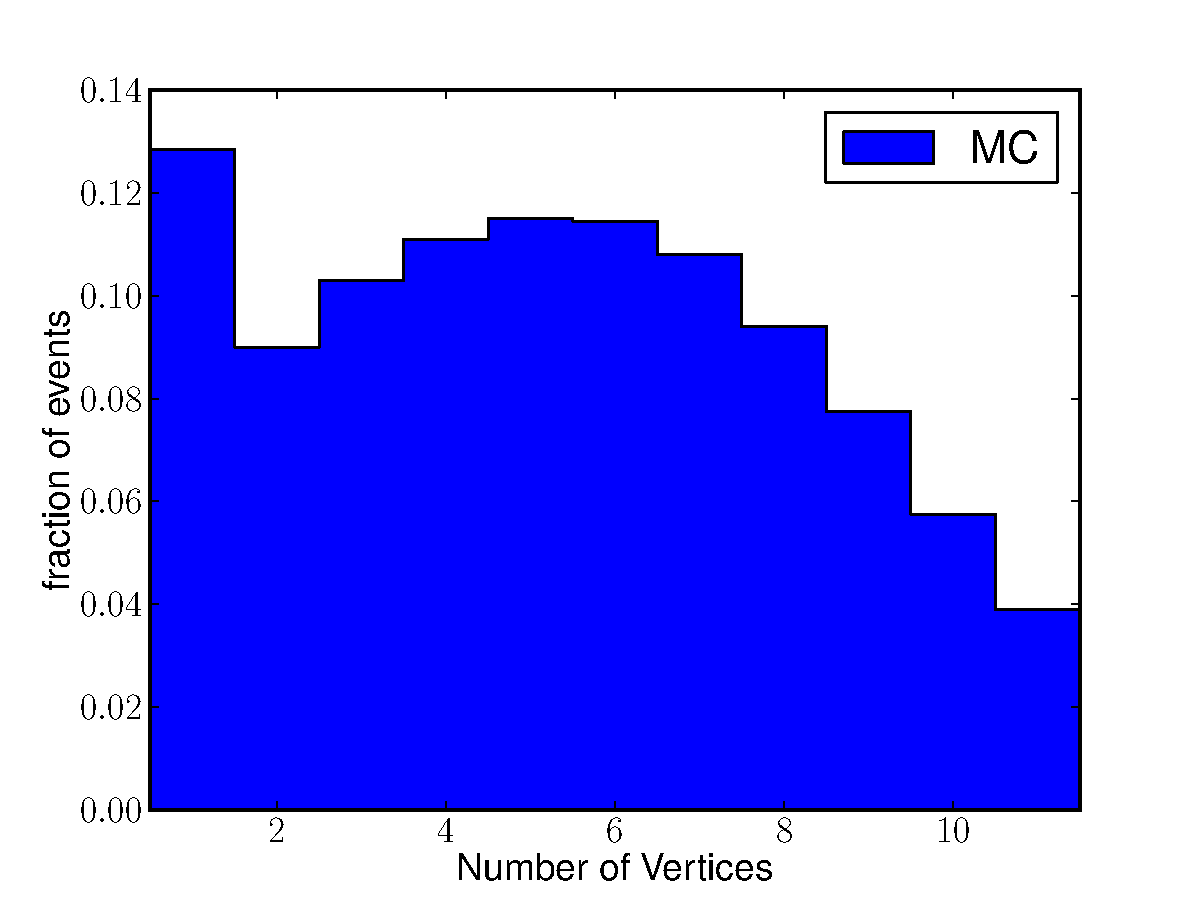
\includegraphics[width=0.5\textwidth]{nVertices_MC.pdf}
\caption{The distribution of number of vertices in the data (left) and the MC
(right).}
\label{fig:nVertices}
\end{figure}

%\begin{table}
%\begin{center}
%{\scriptsize
%\begin{tabular}{|l|c|c|c|c|c|c|c|c|c|c|c|c|c|}
%\hline
%nVertices & 1 & 2 & 3 & 4 & 5 & 6 & 7 & 8 & 9 & 10 & 11 & 12 \\
%\hline
%Weight & 0.15 & 0.82 & 1.41 & 1.79 & 1.71 & 1.38 & 0.97 & 0.64 & 0.40 & 0.22 &
%0.12 & 0.04 \\
%\hline
%\end{tabular}}
%\end{center}
%\caption{Re-weighting factors to be applied to the MC to correctly reproduce the
%number of vertices distribution in the data.}
%\label{tab:factors}
%\end{table}

Figure \ref{fig:Data_vs_MC} shows plots of two variables, $\HT$ and $\MET$,  to 
show how accurately the Monte Carlo models the data. $\HT$ is a measure of the 
energy scale of the event. SUSY events have high $\HT$. $\MET$ is the missing
transverse energy which is the used to distinguish SUSY events from the
background. These variables are defined properly in Sections
\ref{sec:Missing_Transverse_Energy} and \ref{sec:Event_Selection}. The Monte 
Carlo prediction is good for $\HT$, but the $\MET$ distribution is broader in 
the data than the Monte Carlo. This shows that jets with $\pT > 40 \unit{GeV}$
are well described by the Monte Carlo, but lower enregy jets and unclustered
energy are less well modelled. \\

\begin{figure}
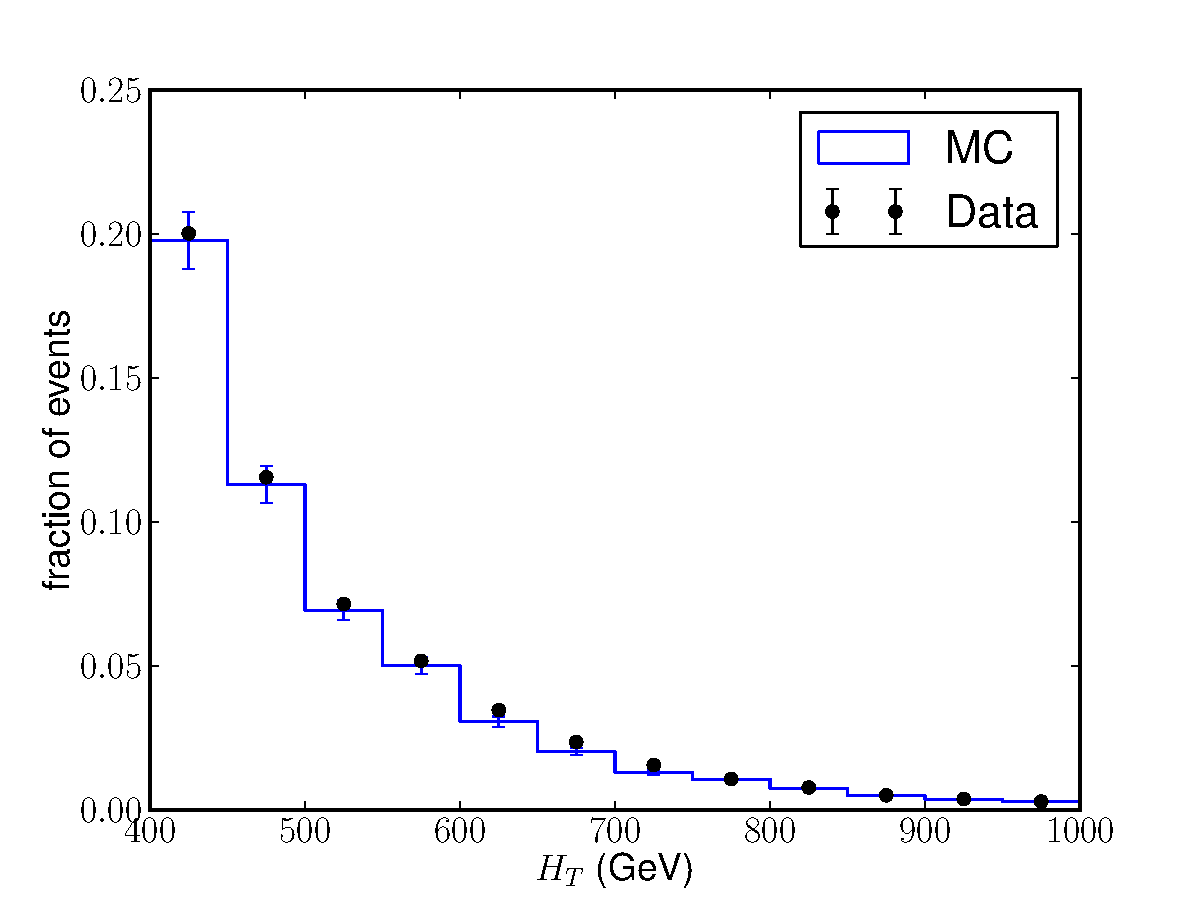
\includegraphics[width=0.5\textwidth]{Data_MC_HT.pdf}
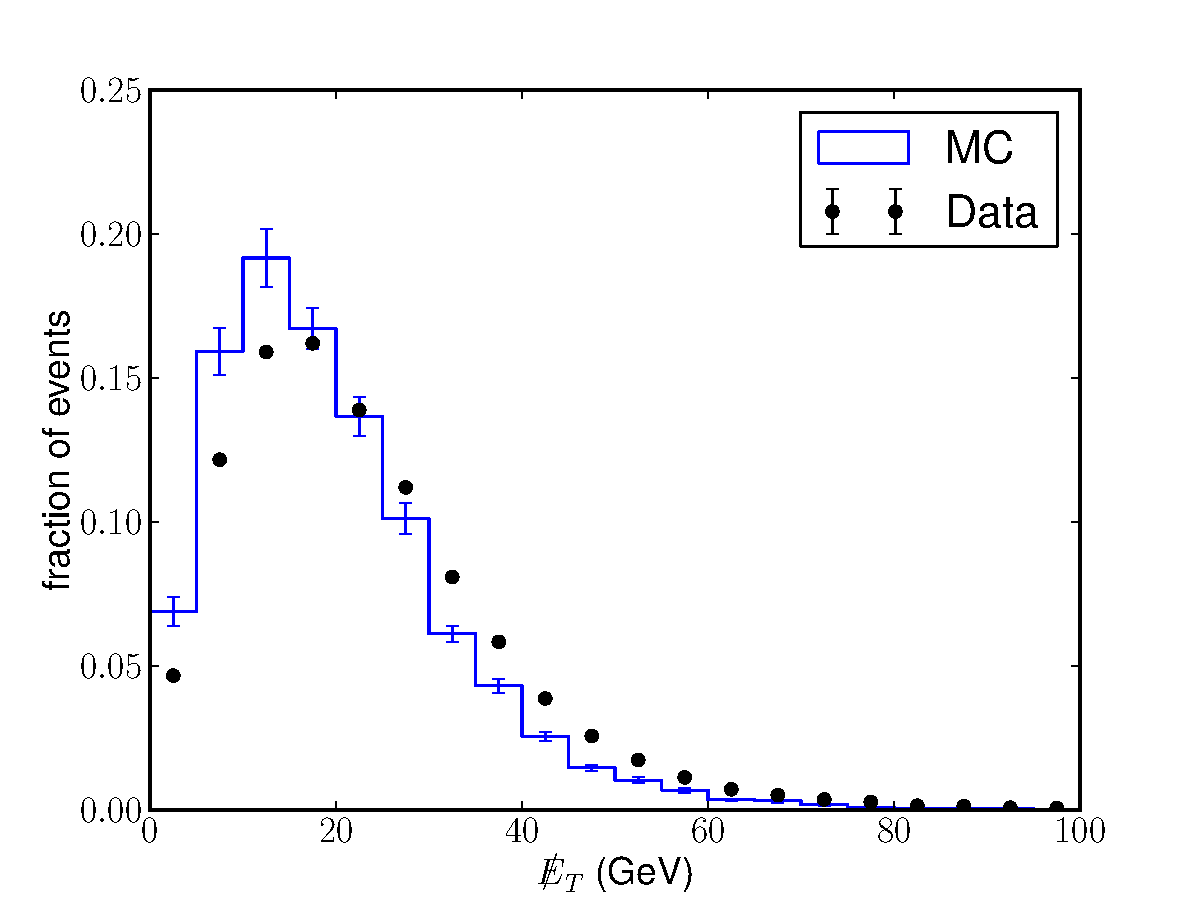
\includegraphics[width=0.5\textwidth]{Data_MC_MET.pdf}
\caption{Plots of $\HT$ and $\MET$ in data and Monte Carlo to show how accurately
the Monte Carlo models the data.}
\label{fig:Data_vs_MC}
\end{figure}

Since the background estimation (see Section \ref{sec:QCD_Background}) is 
largely data-driven the dependence of the result on Monte Carlo is limited.

\section{Trigger}

Based on the properties of strong production GMSB, a photon + $\HT$ trigger 
is ideal for this search. Table \ref{tab:Triggers} shows a list of all the 
photon + $\HT$ triggers in the 2011 data with the corresponding L1 seed and the
rate at $10^{33}\unit{cm^{-2}s^{-1}}$. \\

\begin{table}
\begin{center}
\begin{tabular}{|l|c|c|}
\hline
 & L1 seed & Rate at $10^{33}\unit{cm^{-2}s^{-1}}$ \\
\hline
HLT\_Photon60\_CaloIdL\_HT200 & L1\_SingleEG20 & (pre-scaled) \\
HLT\_Photon70\_CaloIdL\_HT200 & L1\_SingleEG20 & (pre-scaled) \\
HLT\_Photon70\_CaloIdL\_HT300 & L1\_SingleEG20 & $4\unit{Hz}$ \\
HLT\_Photon70\_CaloIdL\_HT350 & L1\_SingleEG20 & $2.5\unit{Hz}$ \\
\hline
\end{tabular}
\end{center}
\caption{A table of the photon and $\HT$ triggers available in the 2011 data
along with the corresponding L1 seed and rate at $10^{33}\unit{cm^{-2}s^{-1}}$.}
\label{tab:Triggers}
\end{table}

As the luminosity has increased more stringent trigger requirements have been 
necessary to keep the data rate manageable. If the rate of a trigger becomes too
high, the trigger must be pre-scaled. This means that only every $n^{th}$ event 
which fires the trigger is read out where $n$ is the prescale factor. \\

The efficiency of a trigger is evaluated with respect to a lower threshold
trigger. Data ranges are selected such that the two triggers are both in the
menu and the higher threshold trigger is unprescaled. To evaluate the trigger
efficiency as a function of $\HT$ the $\HT$ distribution of events passing both
triggers is divided by the $\HT$ distribution of events passing the lower
threshold trigger. The efficiency curve tells us where to put the off-line cut 
in $\HT$ such that the trigger is fully efficient. \\

The efficiency is determined over the run ranges where the trigger overlaps with
one of a lower threshold (see Figure \ref{fig:Trigger_vs_Run_Number}). Figure 
\ref{fig:Trigger_Efficiency} shows the trigger efficiency against $\HT$ and 
photon $\pT$.

\begin{figure}
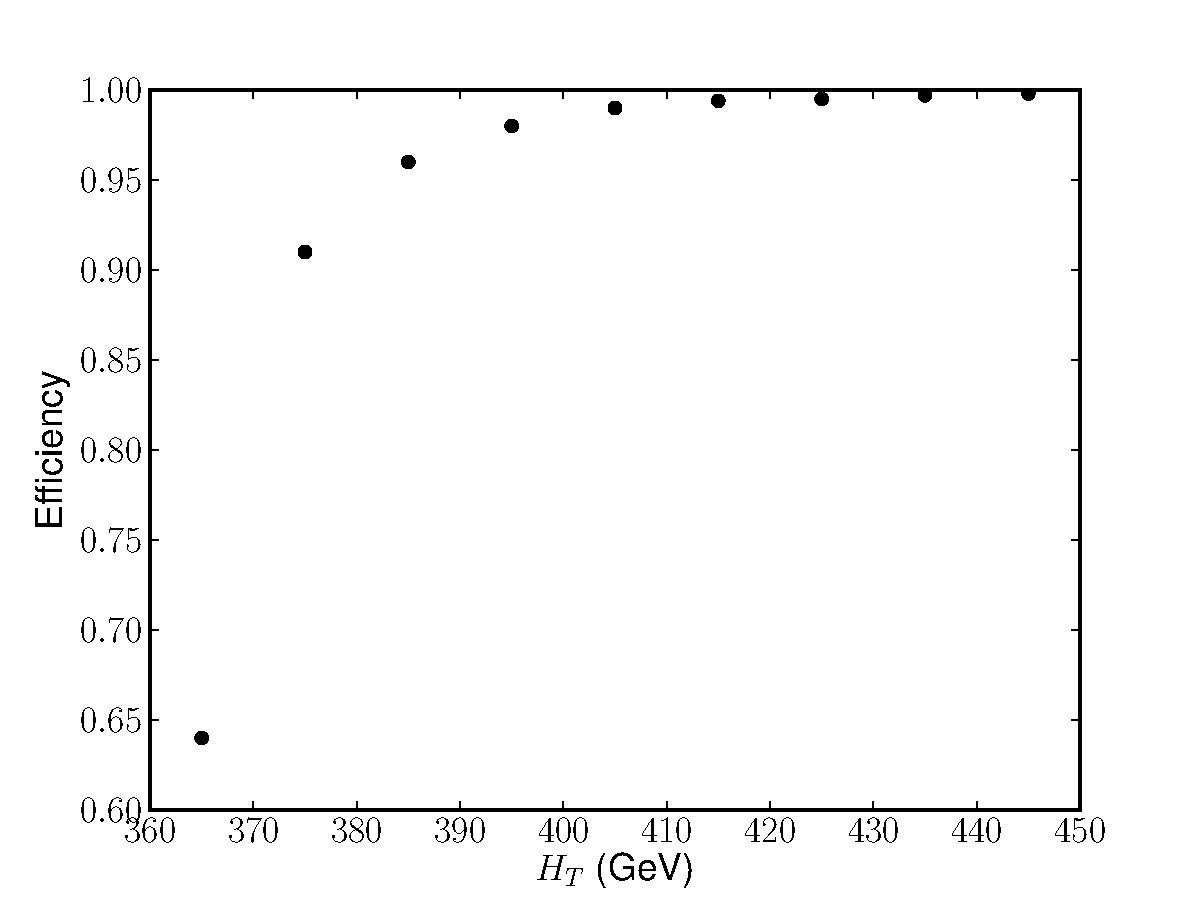
\includegraphics[width=0.5\textwidth]{Trigger_Efficiency_HT.pdf}
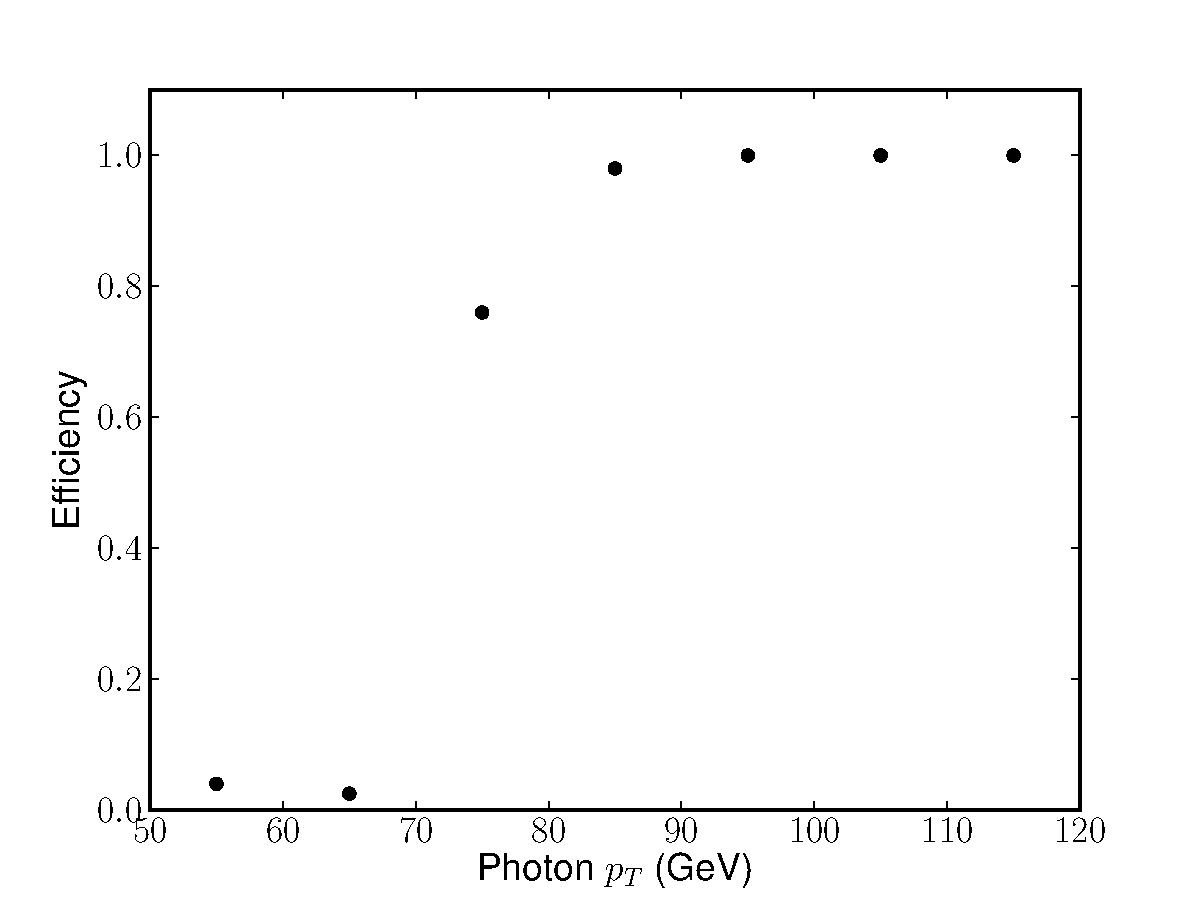
\includegraphics[width=0.5\textwidth]{Trigger_Efficiency_PhotonPt.pdf}
\caption{The trigger efficiency vs $\HT$ (left) and vs photon $\pT$ (right)
relative to a lower threshold trigger.}
\label{fig:Trigger_Efficiency}
\end{figure}

\section{Photon Selection}

Photons are selected based on variables such as isolation and shower shape which
are designed to select prompt photons over fakes from jets. The photon 
reconstruction is described in detail in Section \ref{sec:photon_recontruction}. 
The cut values on each of the photon selection varaibles are listed in Table 
\ref{tab:photoncuts}. 

\begin{table}
\begin{center}
\begin{tabular}{|c|c|}
\hline
Variable & Cut value \\
\hline
ECAL isolation & $4.2 + 0.006\pT$ \\
HCAL isolation & $2.2 + 0.0025\pT$ \\
Track isolation & $2.0 + 0.001\pT$ \\
H/E & 0.05 \\
Shower Shape & 0.012 (EB), 0.030 (EE) \\
No Pixel Seed & True \\
\hline
\end{tabular}
\end{center}
\caption{The photon selection cuts.}
\label{tab:photoncuts}
\end{table}

\section{Jet Selection}

Two jets with $\pT > 80 \unit{GeV}$ and $|\eta| < 2.5$ are required. The $\eta$
threshold corresponds to the tracker boundary. The $\pT$ threshold should be
chosen as high as possible to reject background, but with the signal efficiency
close to 100\%. Figure \ref{fig:Jet_Threshold} shows the signal efficiency and 
the background rejection as a function of the jet $\pT$ threshold. 

\begin{figure}
\begin{center}
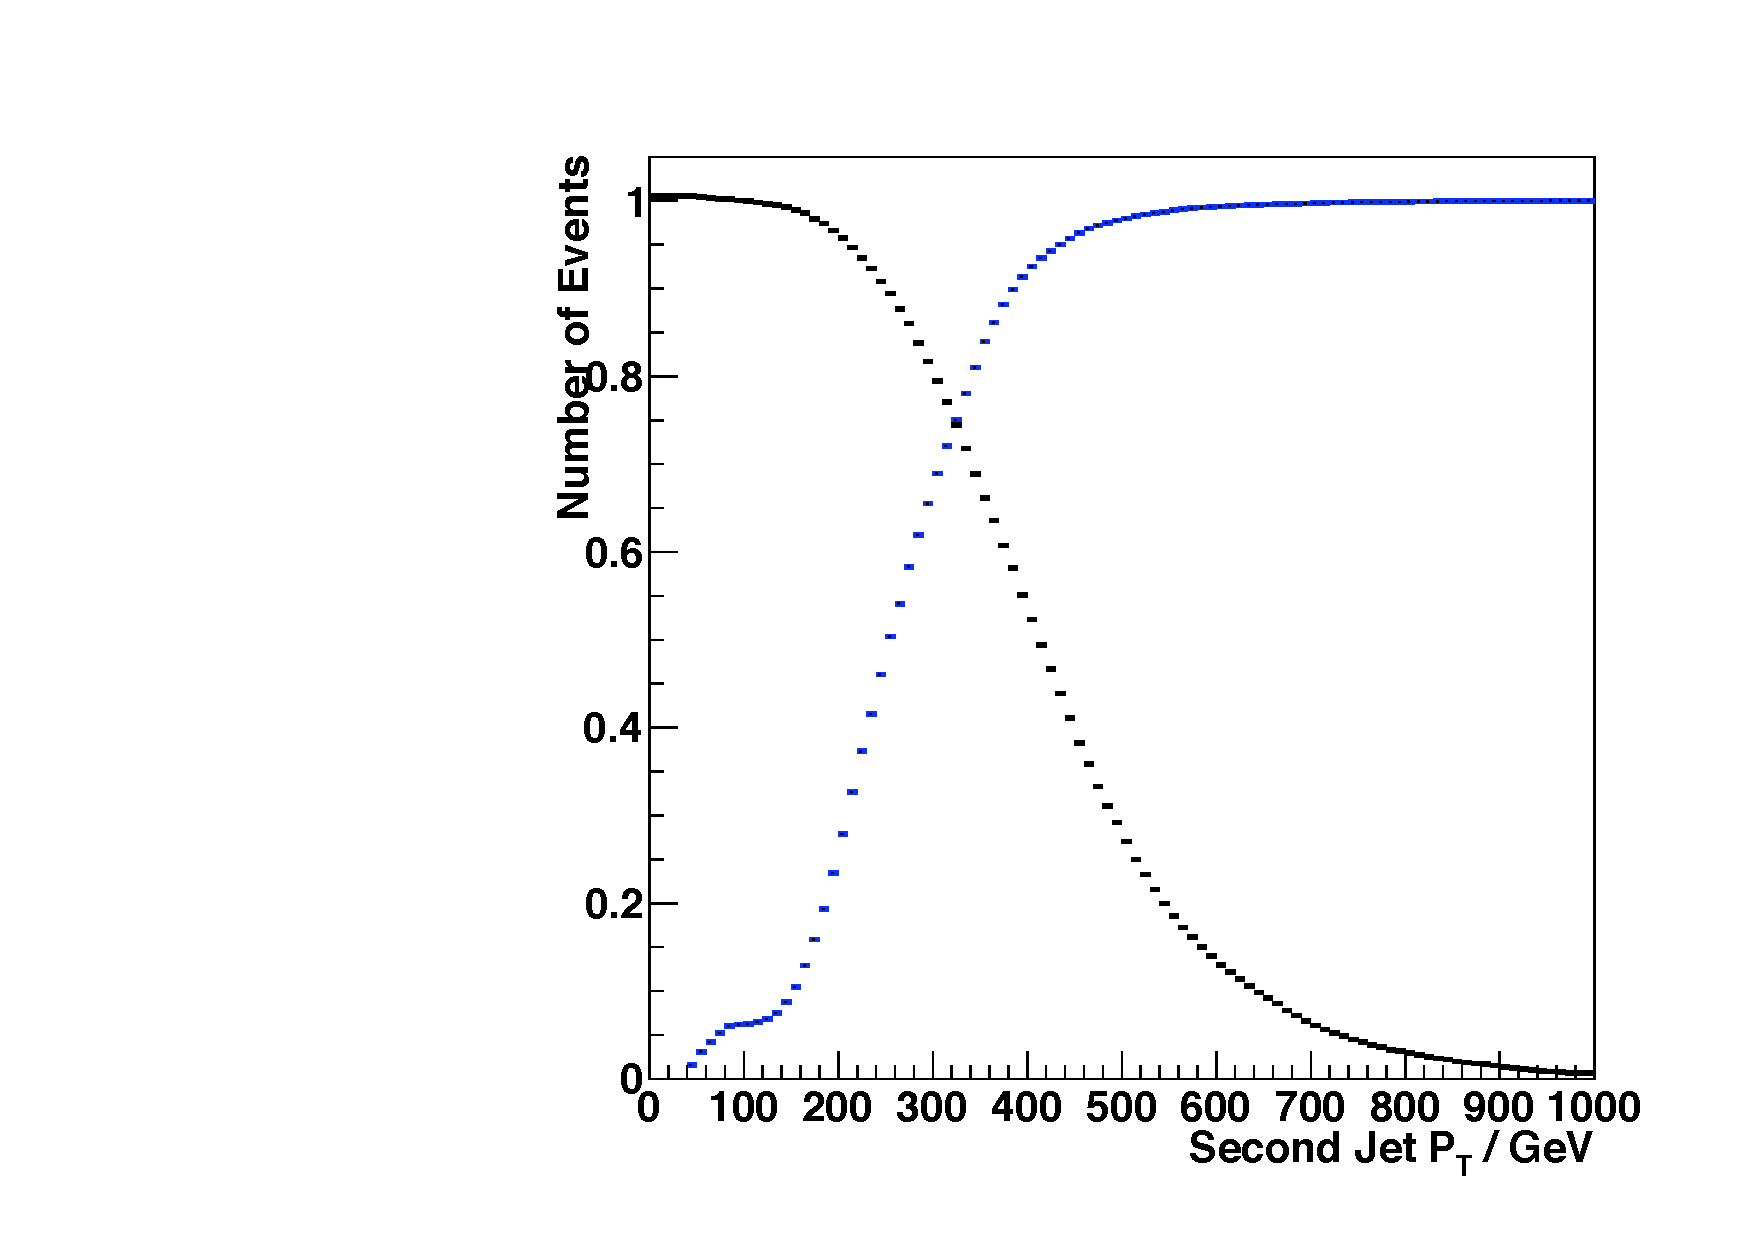
\includegraphics[width=0.7\textwidth]{Jet_Threshold.pdf}
\end{center}
\caption{A plot of the efficiency of the signal (black) and the background
rejection (blue) as a function of the jet $\pT$ threshold.}
\label{fig:Jet_Threshold}
\end{figure}

\section{Missing Transverse Energy}
\label{sec:Missing_Transverse_Energy}

By conservation of momentum, the sum of the momenta of all the final state
particles in a collision is equal to the sum of the momenta of all the inital
state particles. The initial longitudinal momentum of the colliding partons is
unknown since the fraction of the proton momentum that each parton carries is
unknown for any individual event. However, the initial transverse momentum is
known to be close to zero so the final transverse momentum must also be close to 
zero. \\

The missing transverse energy is calculated using the sum of the transverse
momentum of the reconstructed particles. For high energy photons and jets, the 
most accurate determination of the momentum comes from the energy measurement in
the calorimeters. The transverse energy of an energy deposit E is calculated as 
in Equation \ref{eq:et}. The missing transverse energy is calculated as the
negative sum of the transverse energies of all the energy deposits (Equation
\ref{eq:met}). \\

\begin{equation}
\overrightarrow{\ET} = E\sin{\theta}\cos{\phi}\vec{x} + E\sin{\theta}\sin{\phi}\vec{y}
\label{eq:et}
\end{equation}

\begin{equation}
\overrightarrow{\MET} = - \sum \overrightarrow{\ET}
\label{eq:met}
\end{equation}

Events with small missing transverse energy are to be expected because of the 
detector resolution part of which comes from fluctuations inherent in the 
hadronic shower. Missing transverse energy from these sources is expected to be 
gaussian distributed in x and y. Large missing transverse energy can also come 
from undetected particles e.g. neutrinos or detector imperfections e.g. dead 
cells. \\

Motivated by SUSY, this search is based on missing energy. In R-parity
conserving SUSY models events have decay chains ending in the Lightest 
Supersymmetric Particle (LSP) which goes undetected and hence shows up as 
missing transverse energy. In contrast, QCD events (which are the dominant 
background) have only fake missing energy due to detector imperfections. \\

\section{Event Selection}
\label{sec:Event_Selection}

The event selection criteria are listed below. 

\begin{itemize}
\item Noise Cleaning
\item $\HT > 400 \unit{GeV}$
\item $\geq 2$ jets
\item $\geq 1$ photon
\item $\MET > 50 \unit{GeV}$
\end{itemize}

Threee types of noise cleaning are applied to the events. 
\begin{itemize}
\item {\bf Primary Vertex Selection:} Events are required to have at least one
Primary Vertex with $|z| < 24\unit{cm}$, $\mbox{nDOF} > 4$ and $\rho <
2\unit{cm}$.
\item {\bf HCAL Noise Filter:} There are three types of HCAL noise: HPD noise, 
RBX noise and PMT window noise. HPD noise comes from the hybrid photodiodes in
the HB, HE and HO. Misalignment between the HPD electric field and the external
magnetic field can lower the flashover voltage of the HPD resulting in 
occasional cascades where all or most of the 18 channels within the HPD report
large energy deposits. RBX noise is when all or most of the 72 channels in a
Readout Box report large energies. The origin of this noise is cross-over in the
electronics where a signal causes an induced signal in neighbouring wires.
PMT window noise comes from charged particles occasionally hit an HF PMT window 
directly instead of interacting with the quartz fibres. The HCAL noise filter 
removes HCAL noise by vetoing on variables related to pulse shape, timing, hit 
multiplicity and number of zero ADC counts.
\item {\bf ECAL Spike Cleaning:} ECAL Spikes are isolated energy deposits in 
the ECAL which do not come from EM showers. The origin of ECAL spikes is pions
going directly into the depleted region of the photodetector (without
interacting in the ECAL) making it look like there is a significant energy 
deposit in the ECAL. ECAL spikes lead to fake photons and fake MET. There are 
two properties which characterise ECAL spikes: topology and timing. ECAL spikes 
tend to be single crystal enrgy deposits in the ECAL which are often not vetoed 
by the shower shape variable. Some spikes occur at the same time as the bunch
crossing while some occur between bunch crossings. The energy varies from a few 
MeV to a few TeV. A cut of $1 - e4/e1 < 0.96$ is made to avoid ECAL Spikes. 1 - 
e4/e1 is the ``Swiss Cross'' variable in which e1 is the highest energy crystal 
in a 3x3 array and e4 is the energy of the four adjacent crystals. Remaining 
spikes are vetoed by requiring $e2/e9 < 0.96$ and $|t| < 5\unit{ns}$, t is the 
timing of the signal. e2 is the energy of the highest energy crystal plus the
energy of the highest energy adjacent crystal in a 3x3 array. e9 is the total
energy of all the crystals in the 3x3 array. This is illustrated by Figure 
\ref{fig:spikes}.
\end{itemize}

\begin{figure}
\begin{center}
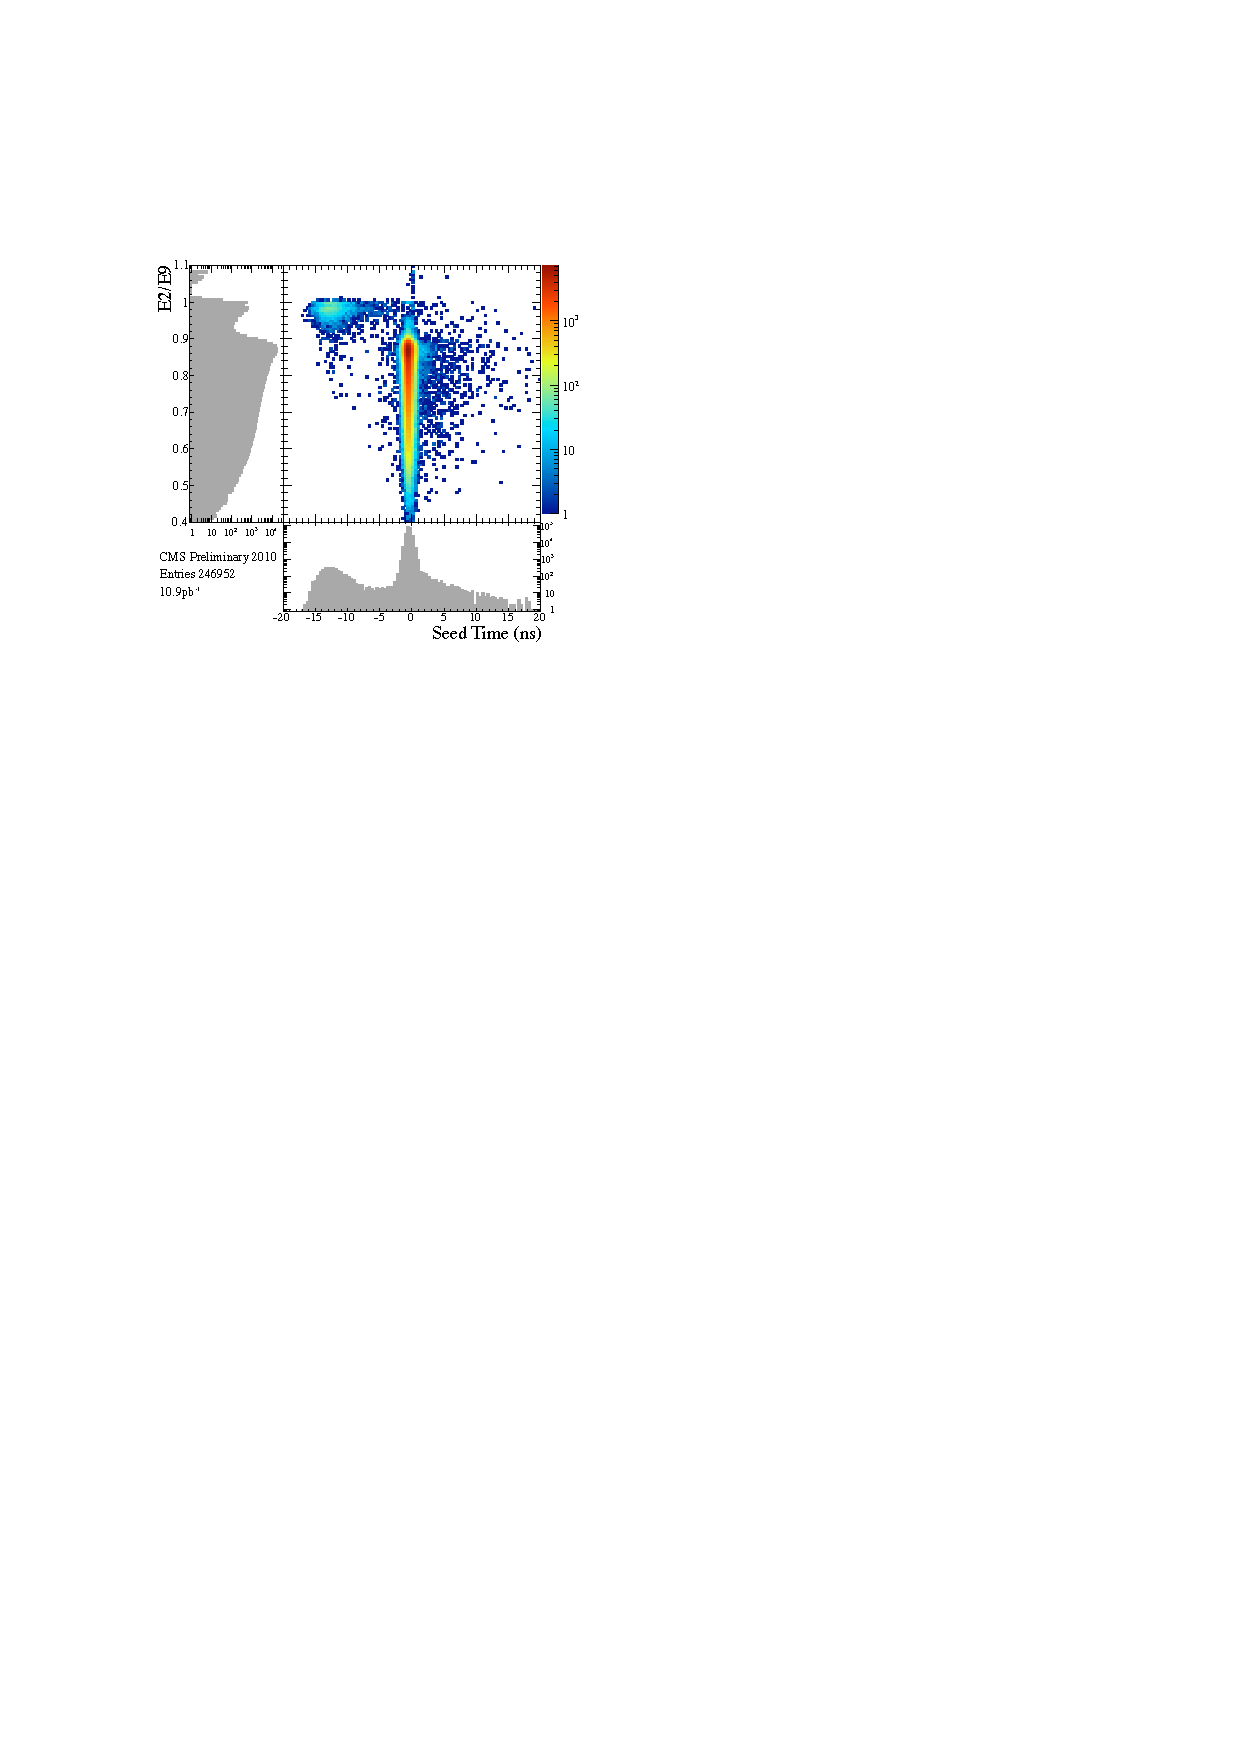
\includegraphics[width=\textwidth]{spikes.pdf}
\end{center}
\caption{A plot of e2/e9 vs seed time to show how double crystal ECAL spikes are
vetoed.}
\label{fig:spikes}
\end{figure}

$\HT$, the scalar sum of the transverse momentum of all the objects in the 
event, is used as a measure of the energy scale of the event. Strongly produced 
SUSY events have high $\HT$ because high mass particles are produced (squarks
and gluinos) which decay hadronically. The value of this cut is motivated by the 
desire for the trigger to be fully efficiency for the event selection. Figure 
\ref{fig:Trigger_Efficiency} shows that the trigger becomes fully efficient in
$\HT$ at around $400\unit{GeV}$. \\

The $\geq 2$ jets cut is well motivated from the SUSY perspective: strongly
produced SUSY events start with two squarks/gluinos each of which decay to a 
quark/gluon (which forms a jet in the detector) and the next SUSY particle in 
the mass hierarchy. \\

In strongly produced Gauge Mediated SUSY Breaking the Next-to-Lightest SUSY 
Particle (NLSP) is the neutralino ($\tilde{\chi}^{0}$) which decays to a photon 
and a gravitino. At least two photons are expected in each event. However, due 
to the high activity in these events, photons often fall inside the cone of a 
jet and so only one photon is reconstructed. Hence the $\geq 1$ photon cut. \\

The search is done in bins of $\MET$ and $\HT$, but an initial $\MET$ cut is
made to avoid the low $\MET$ bins where there is no sensitivity due to the huge
amount of background. Figure \ref{fig:met_threshold} shows the signal efficiency
and the background rejection as a function of $\MET$ cut.

\begin{figure}
\begin{center}
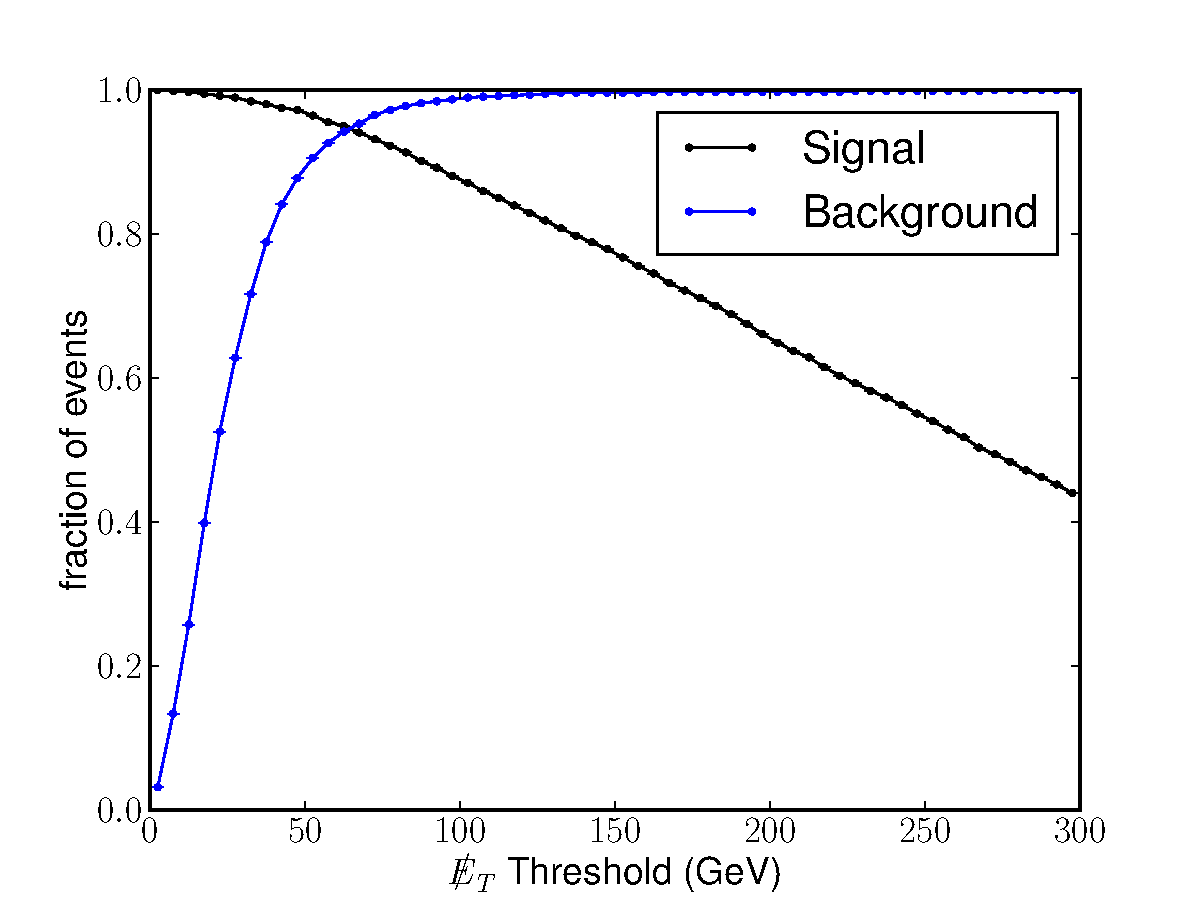
\includegraphics[width=0.7\textwidth]{MET_Threshold.pdf}
\end{center}
\caption{The signal efficiency (black) and background rejection (blue) as a
function of $\MET$ cut.}
\label{fig:met_threshold}
\end{figure}

The total number of events passing the selection in bins of $\HT$ and $\MET$ is
given in Table \ref{tab:events}.

\begin{table}
\begin{center}
\begin{tabular}{|c|c|c|c|c|}
\hline
$\MET\downarrow | \HT\rightarrow$ & $400-500\unit{GeV}$ & $500-600\unit{GeV}$ 
& $600-700\unit{GeV}$ & $700\unit{GeV}+$ \\ 
\hline
$50-100\unit{GeV}$ & 835 & 591 & 398 & 609 \\
\hline
$100-150\unit{GeV}$ & 35 & 30 & 26 & 44 \\
\hline
$150-200\unit{GeV}$ & 5 & 5 & 2 & 7 \\
\hline
$200\unit{GeV}+$ & 9 & 4 & 4 & 7 \\
\hline
\end{tabular}
\end{center}
\caption{The number of events passing the selection in bins of $\HT$ and $\MET$.}
\label{tab:events}
\end{table}
